\section{Implementation und Tests}

%TODO vielleicht
%\subsection{Apps}
%Bei Django werden unabhängige Funktionalitäten in unterschiedliche Apps aufgeteilt. Eine App in Django ist eigentlich nichts anderes als ein Python Package, welches eine Reihe von Features zur Verfügung stellt\footcite{django:apps}. Das Ziel dabei ist es, den Code auf die verschiedenen Apps aufzuteilen, so dass diese unabhängig voneinander wiederverwendet werden können.  \\
%In der Tabelle \ref{table:django_apps} sind die einzelnen Apps aufgelistet, welche für Aufgaben-Coaching erstellt wurden.
%
%\begin{table}[h]
%	\centering
%	\begin{tabu} to 0.9\textwidth {l X}
%	\toprule
%	App & Beschreibung \\ 
%	\midrule	
%	user & In der Users App befindet sich die gesamte Logik zum erstellen und verwalten der User. \\
%	\midrule
%		school\_admin & Die school\_admin App ist für die Erstellung von Klassen sowie der Zuweisung von Schülern und Lehrern in Klassen zuständig. \\
%	\midrule
%	school\_teacher & In dieser App können Lehrer die Fächer für ihre Klasse freischalten und Aufgaben dem Wochenplan hinzufügen. \\
%	\midrule
%		exercise & Die exercise App stellt um Aufgaben zu erstellen zur Verfügung. Zudem können gelöste Aufgaben von einem Lehrer bewertet werden. \\
%	\midrule 
%	study\_content & Diese App beinhaltet die Logik zum bereitstellen von Lerninhalten \\
%	\midrule	
%	forum & In der forum App wird die komplette Logik für das Forum implementiert. \\
%	\bottomrule
%	\end{tabu}
%	\captionof{table}{Apps Beschreibung}
%	\label{table:django_apps}
%\end{table}




\subsection{Testing}
Folgende Tests wurden durchgeführt, um die Qualität dieser Arbeit zu gewährleisten:

\subsubsection*{Unit Tests}
Anhand der Unittests werden die erstellten Models getestet.

\subsubsection*{Integration Tests}
Mit Integration Tests kann getestet werden, ob die Applikation koorekt auf eingehende Requests reagiert.

\subsubsection*{Manuelle Tests}
Diese Tests werden da eingesetzt, wo das erstellen von Tests sehr schwierig oder Zeitaufwändig wäre. So wurde zum Beispiel manuell geprüft, ob das Filtering und Pagination zusammen funktionieren.

\subsubsection*{Usability Tests}
Anhand der Usability Tests soll sichergestellt werden, dass das gewählte Design bei den Mockups einfach und selbsterklärend ist. Hierfür wurden den Probanden einige Aufgaben sowie die erstellen Mockups vorgelegt und darauf geachtet, wie sie sich zurecht fanden.


\subsubsection{Funktionale Tests}
Mit den geschriebenen Tests wurde eine Testcoverage von 97\% erreicht. Bei so hohen Zahlen muss man vorsichtig sein. Nur weil die Testcoverage so hoch ist, heisst es noch lange nicht, dass die Software keine Fehler aufweisst \footcite{test_coverage}. Nur weil eine Zeile Code bei einem Test durchlaufen wird, bedeutet das nicht, dass die Zeile auch getestet wurde. Grundsätzlich gibt es zwei grosse Fehler, die man beim Testen machen kann. Der erste Fehler ist es eine Testcoverage von 100\% anzustreben und sich einZUreden, dass der Code einwandfrei getestet wird. Der zweite Fehler ist es, keinen Wert auf die Testcoverage zu legen. Erreicht man Werte im Bereich von 30\% bis 40\%, ist sofort klar, dass das Testen vernachlässigt wurde. Im allgemeinen gilt, die Qualität der Tests ist ausschlaggebend. Eine hohe Testcoverage erreicht durch sinnvolle Tests ist daher ein anzustrebendes Ziel. 

\textbf{Unittests:} \\
Mithilfe der Unittests werden die Models getestet. Hierbei wird Wert darauf gelegt, dass die Models so reagieren, wie sie reagieren sollen. Es soll also zum Beispiel sichergestellt werden, dass ein Objekt als String so repräsentiert wird, wie es erwartet wird. Zusätzlich soll getestet werden, dass nicht mehrere gleiche Objekte erstellt werden können. Wenn in der Datenbank bereits ein Subject mit dem Titel ''Mathematik'' existiert, soll sichergestellt werden, dass kein weiteres mit dem selben Titel erstellt werden kann.

\textbf{Integration Tests:} \\
Da die Applikation von drei verschiedenen Benutzergruppen verwendet wird, wurde besonders grossen Wert darauf gelegt zu prüfen, dass jeder Nutzer nur im Rahmen seiner vorbestimmten Rechte agieren kann. Es soll einem Schüler zum Beispiel nicht möglich sein, abgegebene Aufgaben zu bewerten, oder eine bereits gemachte Bewertung anzupassen. Aus Erfahrung kann gesagt werden, dass es bei Schülern im Alter von sechs bis sechzehn Jahren nicht besonders lange dauert, bis die ersten Versuche unternommen werden. Würde es Schülern gelingen selber Bewertungen vorzunehmen, würde dies die genrierten Statistiken verfälschen, wodurch ein wichtiger Bestandteil der Applikation seinen Sinn verlieren würde, was auf jeden Fall vermieden werden sollte. 

\textbf{Manuelle Tests:} \\
Es wurde entschieden, dass jedes mal bevor ein Branch mit neuen Funktionen in den Master-Branch gemerget werden soll, zuerst manuelle Tests durchgeführt werden müssen. Alle bis dahin implementierten Funktionen mussten vollständig manuell getestet werden. Dies ist eine wichtige Massnahme, da Funktionen wie zum Beispiel das Filtern der abgegebenen Aufgaben, oder das verschieben von Elementen per Drag\&Drop schwer mit Unittests zu testen sind. Wurde ein Fehler entdeckt, musste dieser sofort behoben und das mergen mit dem Master-Branch solange verschoben werden.



\subsubsection{Usability Tests}
Die Usability Tests wurden mit den in der Planung erstellen Mockups durchgeführt. Die Mockups wurden mit der Webapplikation Balsamiq \footcite{balsamiq_mockups} erstellt. Bereits während des Engineering Projekts und der Studienarbeit konnten damit Erfahrungen gesammelt werden. Zudem ermöglicht es Balsamiq relativ leicht, schöne interaktive Mockups zu erstellen. Durch interaktive Mockups kann die Qualität der Usability Tests verbessert werden, da es sich für die Probanden echter anfühlt und sie dadurch mit grösserer Wahrscheinlichkeit so reagieren, wie sie es dann auf der effektiven Webseite tun werden \footcite{interactive_mockups}. \\

Um möglichst realitätsgetreue Tests durchzuführen, wurden die Probanden gebeten, die Usability Tests dreimal durchzuführen. Bei jeder Durchführung sollen sie eine andere Rolle einnehmen und andere Aufgaben lösen. Um zu verhindern, oder zumindest die Verfälschung der Tests zu minieren, welche durch das gesammelte Wissen vorheriger Durchführungen entstehen kann, wurden die Rollen pro Proband in einer unterschiedlichen Reihenfolge zugweisen. In der Tabelle \ref{Usability Test Rollen} ist ersichtlich, dass drei Probanden die Tests durchgeführt haben und welche Rolle sie bei welcher Durchführung zugewiesen bekommen haben. \\

\begin{table}[h]
	\centering
	\begin{tabu} to 0.9\textwidth {l X X X}
	\toprule
		Proband & Durchführung 1 & Durchführung 2 & Durchführung 3 \\ 
	\midrule
		Proband 1 & Schüler & Lehrer & Administrator \\
		Proband 2 & Lehrer & Administrator & Schüler \\
		Proband 3 & Administrator & Lehrer & Schüler \\
	\bottomrule
	\end{tabu}
	\captionof{table}{Usability Test Rollen}
	\label{Usability Test Rollen}
\end{table}


Beim Durchführen der Usability Tests wurden die Probanden gebeten, beim lösen der Aufgaben laut zu denken. Während der Durchführung wurden anhand der Gedanken und Anmerkungen der Probanden Notizen aufgeschrieben. Da die verschiedenen Benutzergruppen die Applikation später auf unterschiedlichen Geräten verwenden werden, wurde dies in die Tests miteinbezogen. Es wird davon ausgegangen, dass die Schüler die Webapplikation später meistens per Smartphone besuchen werden. Bei den Lehrern und den Administratoren wird davon ausgegangen, dass diese die Webapplikation ausschliesslich per Desktop-PC verwenden. \\

Nachfolgend sind die Aufgaben und Fragen aufgelistet, welche die Probanden pro Rolle lösen/beantworten mussten:

Schüler: \\
\begin{itemize}
	\item Welche Aufgabe/Aufgaben muss/müssen bis am Dienstag erledigt werden?
	\item Navigiere zum ersten Theorieteil des Themas Brüche.
	\item Löse die Aufgabe 1 des Themas Brüche.
	\item Navigiere ins Forum der Aufgabe ''Aufgabe 1'' des Themas Brüche.
	\item Wie kann eine Hilfestellung bei einer Aufgabe angefordert werden?
	\item Wo befindet sich das Quiz 1 des Themas Brüche?
\end{itemize}


Lehrer: \\
\begin{itemize}
	\item Wie sieht der Wochenplan der Klasse ''S2'' aus?
	\item Wie kann der Wochenplan angepasst werden?
	\item Navigiere ins aufgabenspezifische Forum der Aufgabe ''Aufgabe 1'' des Themas Brüche.
	\item Erfasse eine neue Aufgabe für das Thema Brüche.
	\item Wie und wo kann eine bereits erstellte Aufgabe für andere Lehrpersonen freigeschalten werden?
	\item Lösche das Quiz ''Quiz Basics'' des Themas Brüche.
	\item Erstelle ein neues Quiz für das Thema Brüche mit zwei bereits erstellten Fragen.
	\item Erfasse eine neue Frage für ein Quiz.
	\item Schaue dir die Statistiken an.
	\item Wie gut hat der Schüler ''Philipp Muster'' das Quiz ''Quiz 1'' des Themas Brüche gelöst?
	\item Bei welcher Frage des Quiz 1 des Themas Brüche hatte der Schüler ''Philipp Muster'' die grössten Probleme?
\end{itemize}


Admin: \\
\begin{itemize}
	\item Erstelle eine neue Klasse.
	\item Erstelle einen neuen Schüler oder Lehrer.
	\item Lösche einen Schüler, Lehrer oder eine Klasse.
	\item Wie kann ein Lehrer oder Schüler einer Klasse zugewiesen werden?
\end{itemize} 

\textbf{Feedback} \\
Anhand dem Verhalten und dem persönlichen Feedback der Probanden, konnten folgende Problem erkannt werden:

Schüler: \\
\begin{itemize}
	\item Es fiel den Probanden schwer, die Quizze zu finden. Es wurde erwartet, dass die Quizze zusammen mit den Theorieteilen und Aufgaben aufgelistet werden.
\end{itemize}

Lehrer: \\
\begin{itemize}
	\item Beim anpassen des Wochenplans einer Klasse, wurde angemerkt, dass nicht sofort klar sei, dass man die Klasse, das Fach und das Thema in einem Drop-Down-Menü auswählen muss, damit die gesuchten Aufgaben dargestellt werden. Es wurde erwartet, dass dies einfacher funktionieren würde.
	\item Die Funktion eine erstelle Aufgabe mit anderen Lehrern zu teilen sei schwer zu finden.
\end{itemize}

Beim implementieren der Webapplikation wurden die aus den Usability Tests gewonnenen Kenntnisse miteinbezogen und verbessert. Ausserdem haben sich die Anforderungen an die Arbeit verändert, weshalb die Quizze kein Bestandteil der Applikation mehr sind. Folgende Anpassungen und Entscheidungen wurden gemacht: \\

\begin{itemize}
	\item Da die Quizze nicht mehr Teil der Arbeit sind, hat sich dieses Problem in Luft aufgelöst.
	\item Um das Verwalten einer Klasse zu vereinfachen, wurde entschieden, dass im Gegensatz zu der Ursprünglichen Version sich die entsprechende Seite dynamisch erweitert. Zu Beginn sollen nur die dem Lehrer zugewiesenen Klassen aufgelistet werden. \\
	
\begin{minipage}{\textwidth}
	\begin{figure}[H]
		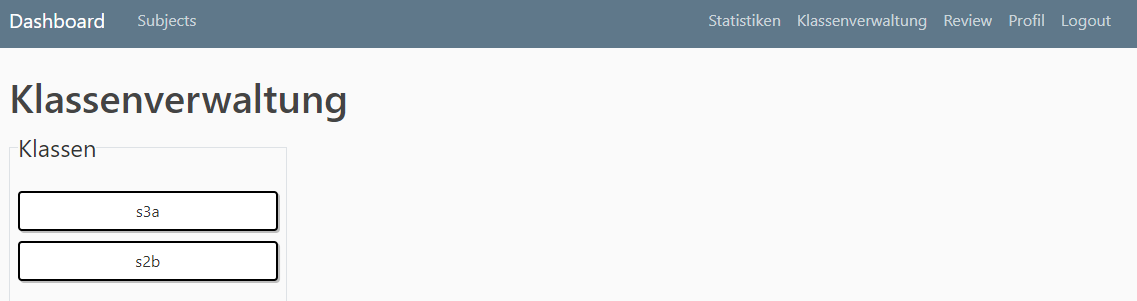
\includegraphics[width=\textwidth, height=\textheight, keepaspectratio]{images/Webseite/Klassenverwaltung_Desktop.png}
		\caption{Anpassung Klassenverwaltung}
	\end{figure}
\end{minipage}	

Nachdem eine Klasse gewählt wurde, werden die klassenspezifischen Informationen geladen und ebenfalls dargestellt. \\

\begin{minipage}{\textwidth}
	\begin{figure}[H]
		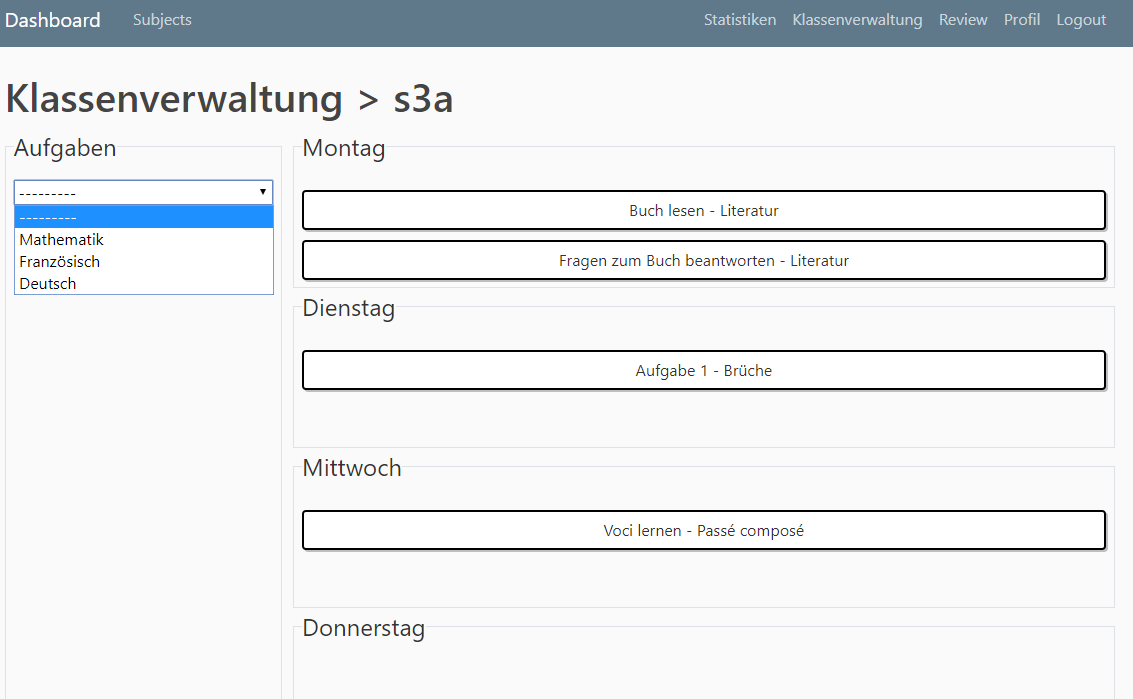
\includegraphics[width=\textwidth, height=\textheight, keepaspectratio]{images/Webseite/Klassenverwaltung_Klasse_Desktop.png}
		\caption{Informationen einer Klasse}
	\end{figure}
\end{minipage}

	\item Die Funktion um eigene Aufgaben mit anderen Lehrpersonen zu teilen wurde entfernt. Standardmässig sind nun alle erstellen Aufgaben für alle Lehrpersonen ersichtlich.
\end{itemize}
